Two main algorithmic approaches are proposed to address the parallel execution of the itemset mining algorithms by means of the MapReduce paradigm. 
They are significantly different because (i) they use different solutions to split the original problem in subproblems and (ii) make different assumptions about the data that can be stored in the main memory of each independent task. 

\begin{description}

\item[Data split approach.]  It splits the problem in ``similar'' subproblems, executing the same function on different data chunks. Specifically, each subproblem computes the local supports of all candidate itemsets on one chunk on the input dataset (i.e., each subproblem works on the complete search space but on a subset of the input data). Finally, the local results (i.e., the local supports of the candidate itemsets) emitted by each subproblem/task are merged to compute the global final result (global support of each itemset). The main assumptions of this approach are that (i) the problem can be split in ``similar' subproblems working on different chunks of the input data and (ii) the set of candidate itemsets is small enough that it can be stored in the main memory of each task.

\item[Search space split approach.]  It splits the problem by assigning to each subproblem the visit of a subset of the search space (i.e., each subproblem visits a part of the lattice). Specifically, this approach generates, from the input distributed dataset, a set of projected datasets, each one small enough to be stored in the main memory of a single task. Each projected dataset contains all the information that is needed to extract a subset of itemsets (i.e., each dataset contains all the information that is needed to explore a part of the lattice) without needing the contribution of the results of the other tasks. The final result is the union of the itemset subsets mined from each projected dataset.

\end{description}


\begin{figure}[!t]
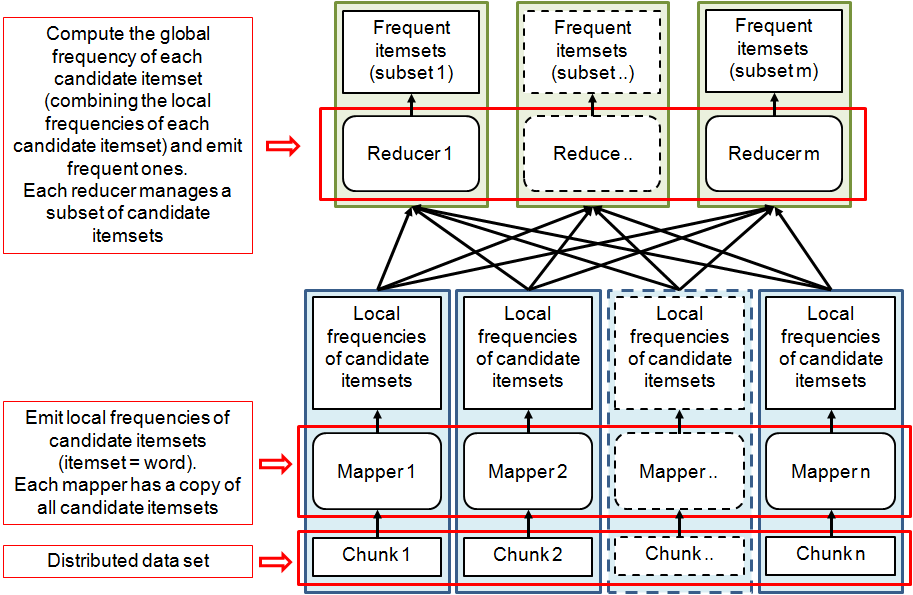
\includegraphics[width=5in]{immagini/Approach1noniterativo.eps}
\caption{Itemset mining parallelization: Data split approach}
\label{approach1noniterativo}
\end{figure}

\begin{figure}[!t]
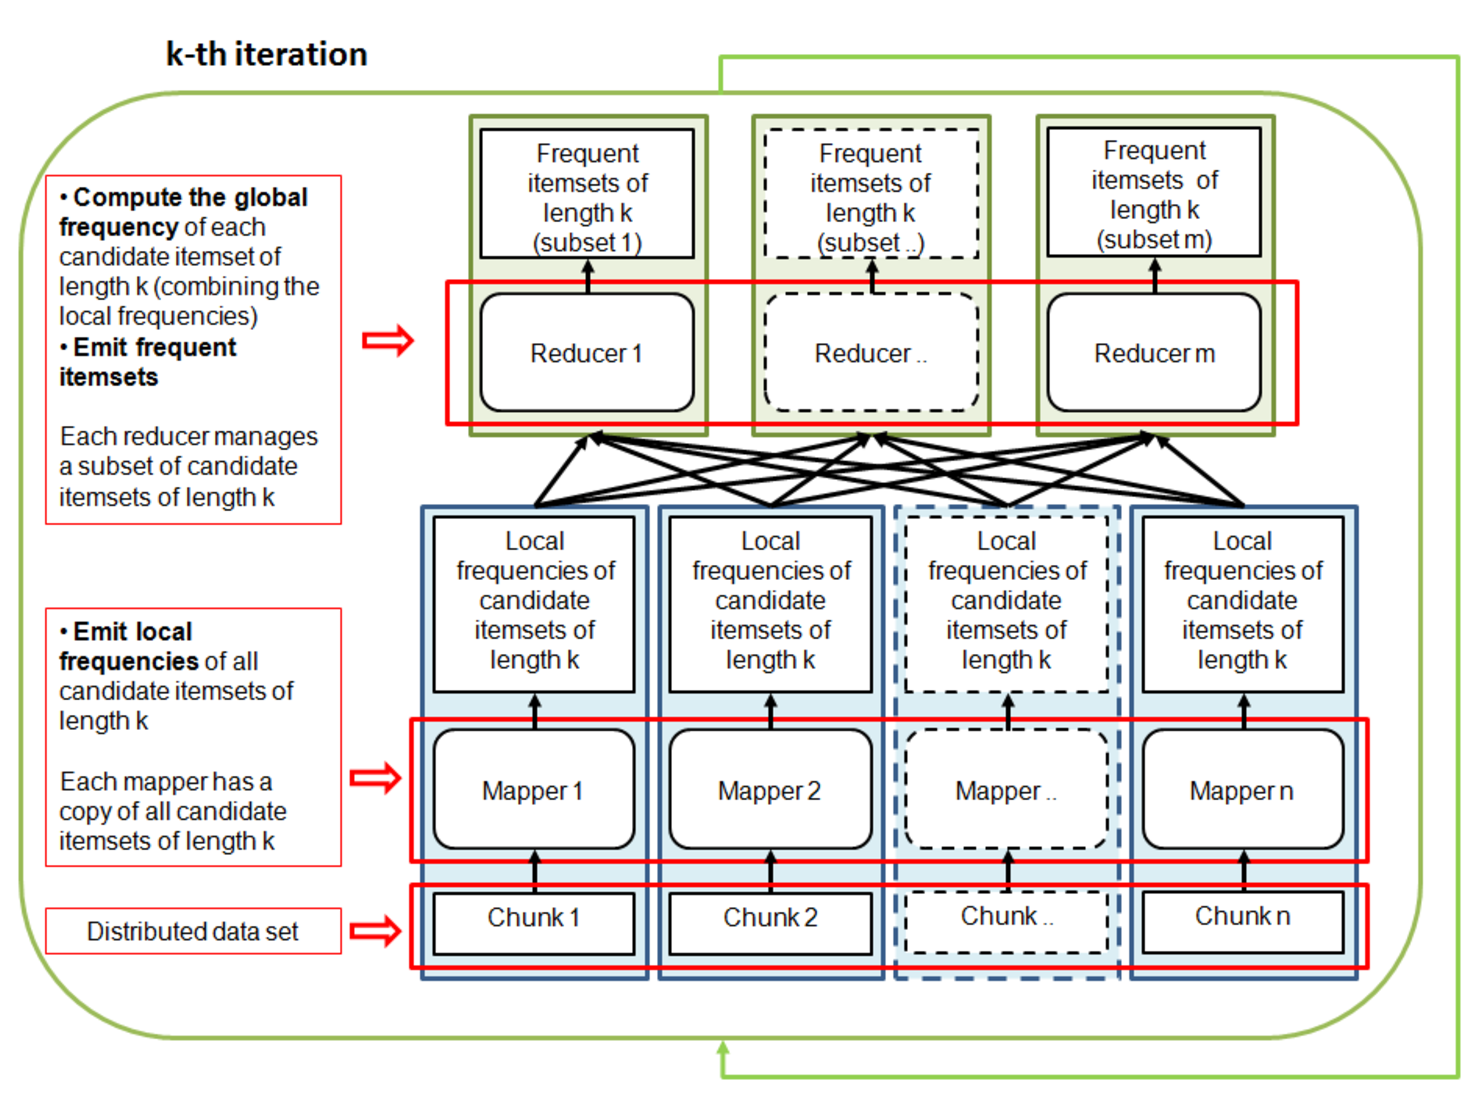
\includegraphics[width=5in]{immagini/Approach1.eps}
\caption{Itemset mining parallelization: Iterative Data split approach}
\label{approach1}
\end{figure}



\begin{figure}[!t]
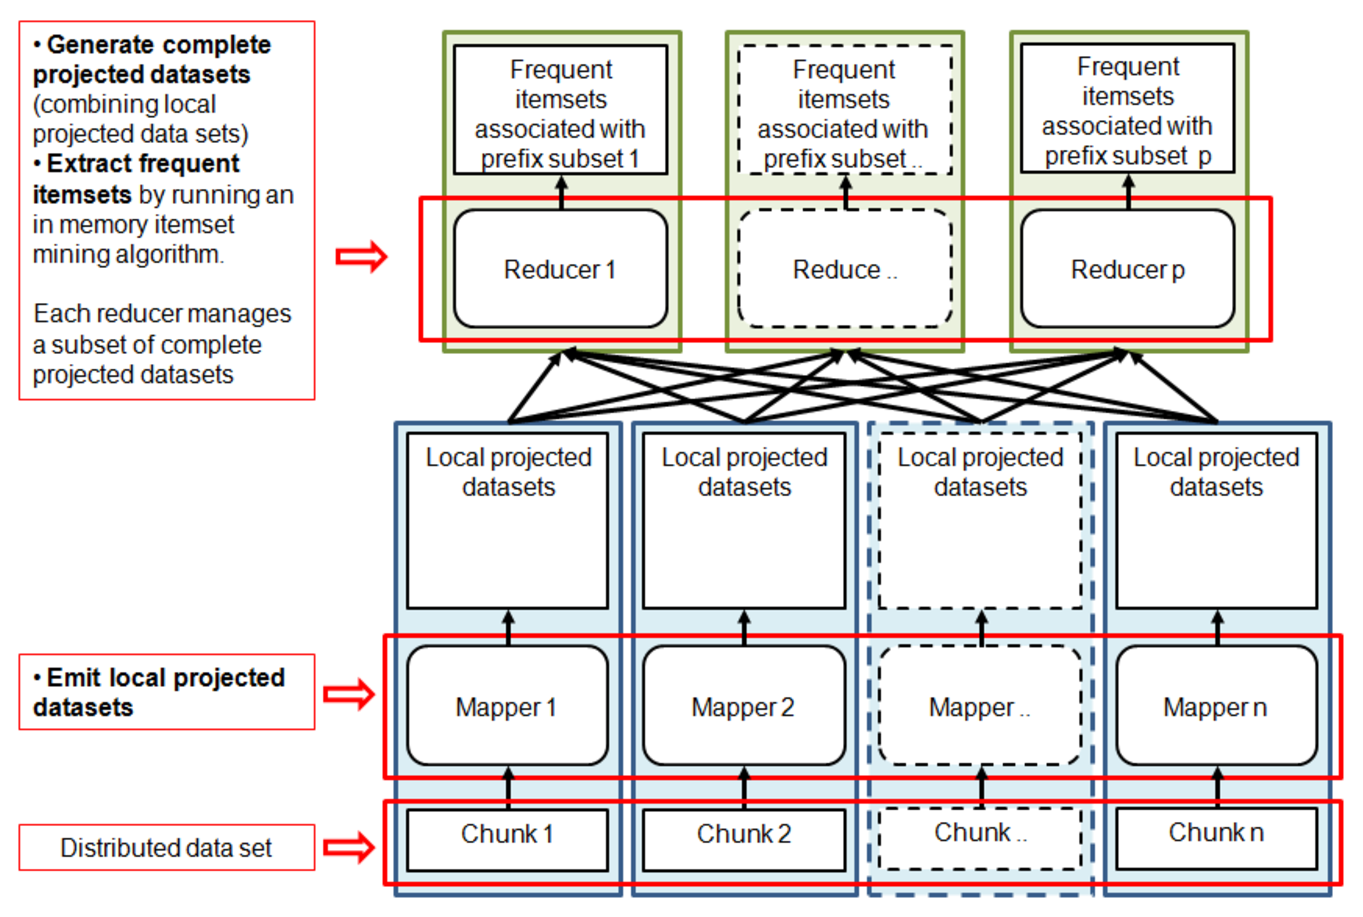
\includegraphics[width=5in]{immagini/Approach2.eps}
\caption{Itemset mining parallelization: Search space split approach}
\label{approach2}
\end{figure}


Figures~\ref{approach1noniterativo} and \ref{approach2} depict the first and the second parallelization strategies, respectively.  
In the data split approach (Figure~\ref{approach1noniterativo}), the map phase computes the local supports of the candidate itemsets in its data chunk  (i.e., each mapper runs a ``local itemset mining extraction'' on its data chunk). Then, the reduce phase merges the local supports of each candidate itemset to compute its global support. This solution requires each mapper to store a copy of the complete set of candidate itemsets (i.e., a copy of the lattice). 
This set must fit in the main memory of each mapper. Since the complete set of candidate itemsets is usually too large to be stored in the main memory of a single mapper, an iterative solution, inspired by the level-wise centralized itemset mining algorithms, is used. Figure~\ref{approach1} reports the iterative solution. 
At each iteration $k$ only the subset of candidates of length $k$ are considered and hence stored in the main memory of each mapper. This approach, thanks also to the exploitation of the apriori-principle to reduce the size of the candidate sets, allows obtaining subsets of candidate itemsets that can be loaded in the main memory of every mapper.

In the search space split approach (Figure~\ref{approach2}), the map phase generates a set of local projected datasets. Specifically each mapper generates a set of local projected datasets based on its data chunk. Each local projected dataset is the projection of the input chunk with respect to a prefix $p$.\footnote{Note that the projected datasets can overlap because the transactions associated with two distinct prefixes $p_1$ and $p_2$ can be overlapped.} Then, the reduce phase merges the local projected datasets to generate the complete projected datasets. Each complete projected dataset is provided as input to a standard centralized itemset mining algorithm running in the main memory of the reducer and the set of frequent itemsets associated to it are mined.
Each reducer is in charge of analyzing a subset of complete projected datasets by running the itemset mining phase on one complete projected dataset at a time.   
Hence, the main assumption, in this approach, is that each complete projected dataset must fit in the main memory of a single reducer. 

Table~\ref{tab:assumptions} summarizes the main characteristics of the two parallelization approaches with respect to the following criteria: 
type of split of the problem, 
usage of main memory, 
communication costs, 
load balancing, 
and maximum parallelization (i.e. maximum number of mappers and reducers).
%These are important issues to be addressed by distributed algorithms to increase their efficiency. 

%The communication cost is the amount of data sent on the network across the nodes of the cluster. The network can quickly  become the bottleneck 
%if large amount of data are sent on it. Hence, appropriate solutions must be adopted to limit it. 
%Load balancing is another important issue. It aims at assigning similar subproblems, characterized by similar execution times, to the nodes of the cluster to maximize the use of the available resources. A well-balanced application allows exploiting, simultaneously, all the available resources, whereas a non-well balanced applications is characterized by busy nodes (the ones associated with the longest tasks) and idle ones (the ones associated with the shortest tasks).

%For completeness, Table~\ref{tab:assumptions} reports both versions of Approach~1. However, the actual implementations are not based on the non-iterative version of Approach~1 because the complete set of itemsets (i.e., the complete lattice) is too large to be stored in main memory.


%\begin{table}[]
%\scriptsize
%\centering
%\caption{Comparison of the parallelization approaches.}\label{tab:assumptions}
%\begin{tabular}{|p{1.5cm}|p{3cm}|p{3cm}|p{3cm}|p{2cm}|}
%\hline {\bf Name} & {\bf Assumption} & {\bf Communication costs} & {\bf Load balancing} & {\bf Number of reads of the distributed dataset} \\
%\hline
%\hline Approach~1 (Figure~\ref{approach1noniterativo})& The complete set of candidate itemsets (i.e., the complete lattice) can be stored in the main memory of a single task. & Number of candidate itemsets $\times$ number of mappers. & Load balancing is achieved by associating the same number of itemsets to each reducer. & 1 \\
%
%\hline Approach~1 - Iterative version (Figure~\ref{approach1}) & Each candidate set of itemsets of length $k$ can be stored in the main memory of a single task. & Number of candidate itemsets $\times$ number of mappers $\times$ number of iterations. & Load balancing is achieved by associating the same number of itemsets to each reducer. & number of iterations (= size of the longest frequent itemset)\\
%\hline Approach~2 (Figure~\ref{approach2})& Each global projected dataset can be stored in the main memory of a single task. & Sum of the sizes of the local projected datasets. & Load balancing is not addressed. The tasks could be significantly unbalanced depending on the difference among the projected datasets and the related mining processes. & 1 \\
%\hline
%\end{tabular}
%\end{table}



\begin{table}[]
\scriptsize
\centering
\caption{Comparison of the parallelization approaches.}\label{tab:assumptions}
\begin{tabular}{|p{2.5cm}|p{5cm}|p{5cm}|}

\hline {\bf Criterion} & {\bf Iterative data split approach (Figure~\ref{approach1})} & {\bf Search space split approach (Figure~\ref{approach2})} \\
\hline
%\hline Type of split/Split of the search space &  All subproblems/mapper tasks analyze all the candidate itemsets of length $k$, but each one works on a different chunk of data. The final result is given by the merge of the local results.  &  Each subproblem analyzes a different subset of itemsets/a different part of the search space. The final result is the union of the local results. \\
\hline Type of split/Split of the search space &  Each subproblem analyzes a different subset of the input data and computes the local supports of 
all the candidate itemsets of length $k$ on its chunks of data. The final result is given by the merge of the local results.  &  Each subproblem analyzes a different subset of itemsets/a different part of the search space. The final result is the union of the local results. \\
\hline Usage of main memory &  The candidate set of length $k$ is stored in the main memory of a single task. & The complete projected dataset is stored in the main memory of a single task. \\
\hline Communication cost &  Number of candidate itemsets $\times$ number of mappers $\times$ number of iterations. & Sum of the sizes of the local projected datasets. \\
\hline Load balancing &  Load balancing is achieved by associating the same number of itemsets to each reducer. & The tasks could be significantly unbalanced depending on the characteristics of the projected datasets assigned to each node.\\
\hline Maximum number of mappers & Number of chunks  & Number of chunks  \\
\hline Maximum number of reducers & Number of candidate itemsets  & Number of items \\
\hline
\end{tabular}
\end{table}

%\begin{table}[]
%\scriptsize
%\centering
%\caption{Comparison of the parallelization approaches.}\label{tab:assumptions}
%\begin{tabular}{|p{2cm}|p{3.4cm}|p{3.4cm}|p{3.4cm}|}
%
%\hline {\bf Criterion} & {\bf Approach~1 (Figure~\ref{approach1noniterativo})} & {\bf Approach~1 - Iterative version (Figure~\ref{approach1})} & {\bf Approach~2 (Figure~\ref{approach2})} \\
%\hline
%\hline Type of split/Split of the search space & All subproblems/mapper tasks analyze all the candidate itemsets (i.e., work on the whole search space), but each one work on a different chunk of data. The final result is given by the merge of the local results.  & All subproblems/mapper tasks analyze all the candidate itemsets of length $k$, but each one work on a different chunk of data. The final result is given by the merge of the local results.  &  Each subproblem analyzes a different subset of itemsets/a different part of the search space. The final result if the union of the local results. \\
%\hline Use of the main memory & The complete set of candidate itemsets (i.e., the complete lattice) can be stored in the main memory of a single task.  &  Each candidate set of itemsets of length $k$ can be stored in the main memory of a single task. & Each global projected dataset can be stored in the main memory of a single task. \\
%\hline Communication costs & Number of candidate itemsets $\times$ number of mappers. &  Number of candidate itemsets $\times$ number of mappers $\times$ number of iterations. & Sum of the sizes of the local projected datasets. \\
%\hline Load balancing & Load balancing is achieved by associating the same number of itemsets to each reducer. &  Load balancing is achieved by associating the same number of itemsets to each reducer. & The tasks could be significantly unbalanced depending on the characteristics of the projected datasets assigned to each node and the related mining processes. Load balancing can not be easily achieved.\\
%%\hline Number of reads of the distributed dataset & 1 & Number of iterations (= size of the longest frequent itemset)  & 1 \\
%\hline Maximum number of mappers & Number of chunks & Number of chunks  & Number of chunks  \\
%\hline Maximum number of reducers & Number of candidate itemsets & Number of candidate itemsets  & Number of items \\
%\hline
%\end{tabular}
%\end{table}


\noindent{\bfseries Type of split/Split of the search space}. 
The main difference between the two parallelization approaches is the strategy adopted to split the problem in subproblems. This choice has a significant impact on the other criteria.

\noindent{\bfseries Usage of main memory}. 
The different usage of the main memory of the tasks impact on the reliability of the two approaches. The data split approach supposes that the candidate itemsets of length k can be stored in the main memory of each mapper. Hence, it is not able to scale on dense datasets
characterized by large candidate sets. Differently, the search space split approach supposes that each complete projected dataset can be stored in the main memory of a single task. Hence, this approach is not adequate, and runs out of memory, when large complete projected datasets are generated.  

\noindent{\bfseries Communication costs}. In a parallel MapReduce algorithm, communication costs are important since the network can easily become the bottleneck if large amounts of data are sent on the network.
The communication costs are mainly related to the outputs of the mappers which are sent to the reducers on the network. 
For the data split approach the data that is sent on the network is linear with respect 
to the number of candidate itemsets, the number of mappers, and the number of iterations.
Differently, for the search space approach, the amount of data emitted by the mappers is equal to the size of the projected datasets. 
%Since the projected datasets are overlapped the result is that the data sent across the network is potentially larger than the initial dataset\footnote{Usually, the size of the data sent on the network is not large as the initial dataset because compact trees are used to represent the projected datasets.}. 


\noindent{\bfseries Load balancing}. 
The different split of the problem in subproblems significantly impacts on load balancing. For the data split approach, the execution time of each mapper 
is linear with respect to the number of input transactions and the execution time of each reducer is linear with respect to the number of assigned itemsets.
Hence, the data split approach can easily achieve a good load balancing by assigning the same number of data chunks to each mapper and the same number of candidate itemsets to each reducer. 
Differently, the search space split approach is potentially unbalanced. In fact, each subproblem is associated with a different subset of the lattice, related to a specific projected dataset and prefix, and, depending on the data distribution, the complexity of the subproblems can significantly vary. 
A smart assignment of a set of subproblems to each node would mitigate the unbalance. However, the complexity of the subproblems is hardly inferable during the initial assignment phase.

\noindent{\bfseries Maximum number of mappers and reducers}. 
The two approaches are significantly different in terms of ``maximum parallelization degree'', at least in terms of number of maximum exploitable reducers. 
The maximum parallelization of the map phase is equal to the number of data chunks for both approaches.
% (i.e., maximum number of mappers = number of data chunks). 
Differently, the maximum parallelization of the reduce phase is equal to the number of candidate itemsets for the data split approach, because potentially each reducer could compute the global frequency of a single itemset, whereas it is equal to the number of global projected datasets for the second approach, which can be at most equal to the number of items. 
Since the number of candidate itemsets is greater than the number of items, the data split approach can potentially reach a higher degree of parallelization with respect to the search space split approach. 


%The communication costs are related to the outputs of the mappers. Since each mapper of the first approach emits one local support for each candidate itemset, the data that is sent on the network is linear with respect to the number of candidate itemsets and the number of mappers.
%Differently, for the second approach, the amount of data emitted by the mappers is equal to the size of the projected datasets. Since the projected datasets are overlapped the result is that the data sent across the network is potentially larger than the initial dataset\footnote{Usually, the size of the data sent on the network is not large as the initial dataset because compact trees are used to represent the projected datasets.}. 
%
%The different split of the problem in subproblems impacts also on load balancing. The first approach can easily achieve load balancing because all mappers perform the same operation and also all reducers perform the same operation. The only difference is given by the input data chunks and input candidate itemsets. By assigning the same number of data chunks to each mapper and the same number of candidate itemsets to each reducer, the result is that all mapper tasks are characterized by a similar execution time and also all reducers are characterized by a similar execution time. This means that the overall application is well-balanced. 
%Differently, the second approach is potentially unbalanced. In fact, each subproblem is associated with a different subspace of the search space, related to a specific projected dataset and prefix, and, depending on the data distribution, the complexity of the subproblems can significantly vary. A smart assignment of a set of subproblems to each node would mitigate the unbalance. However, the complexity of the subproblems is hardly inferable during the initial assignment phase.
%
%
%The two approaches are also different in terms of ``maximum parallelization degree'', at least in terms of number of maximum exploitable reducers. 
%The maximum parallelization of the map phase is equal to the number of data chunks for both approaches (i.e., maximum number of mappers = number of data chunks). Differently, the maximum parallelization of the reduce phase is equal to the number of candidate itemsets for the first approach, because potentially each reducer could compute the final frequency of a single itemset, whereas it is equal to the number of global projected datasets for the second approach, which can be at most 
%equal to the number of items. 
%Since the number of candidate itemsets is greater than the number of items, the first approach can reach a higher degree of parallelization with respect to the second approach. However, pay attention that a higher number of reducers corresponds also to a higher overhead related to the instantiation of the reducers. 

The two parallelization approaches are used to design efficient parallel implementations of well-known centralized itemset mining algorithms.  Specifically, the data split approach is used to implement the parallel versions of level-wise algorithms (like Apriori~\cite{apriori}), whereas the search space split approach is used to implement parallel versions of depth-first recursive approaches (like FP-growth~\cite{Han00} and Eclat~\cite{Zaki97newalgorithms}). 
%The map phase of the second approach can be seen as the first step of the recursion, that is used to generate the datasets projected with respect to prefixes composed of single items. Then, the reduce phase runs, in main memory, one instance of the mining algorithm for each projected dataset.




%{\bfseries Paolo: Capire cosa tenere della parte dopo che era la vecchia versione di questa sezione.}
%
%\textbf{Fabio: la metterei dopo l'intro degli algoritmi} In this section, we describe the main algorithmic solutions that have been exploited to address the
%parallelization of the itemset mining problem in the big data distributed environments (e.g., Hadoop and Spark).
%Many considerations are general and independent of the big data nature of the input data, whereas some other considerations and 
%algorithmic/design choices are driven by the big data characteristics of the input data (e.g., design of algorithms that exploit data locality).
%
%The parallelization and distributed execution of a generic algorithm, in the big data environment, is usually based on the split of the main task 
%in subtasks, each one working in isolation (shared-nothing) on one chunk of the data. However, this approach is not always possible and hence some algorithms 
%share small portions of data among the parallel tasks.
%
%The Hadoop-based algorithms usually parallelize the addressed problems by splitting the input datasets in independent data chucks. 
%Each chuck of the input data is assigned to a subtask that analyses the chunk of data in isolation (i.e., without needing the information 
%available in the other chunks). This is the map phase of the MapReduce programming paradigm. The outputs generated by the subtasks
%are then merged to obtain the final output (i.e., the output of the algorithm applied on the whole data). This second step is the reduce phase.
%The main assumptions of this solution are that (i) the input dataset is big (hence it cannot be sent on the network), whereas the outputs of 
%the subtasks are small and can be sent on the network and shared across the nodes of the cluster and (ii) the initial problem 
%can be split in subproblems each one working on one portion of the data and the portions are not overlapped.
%
%
%The algorithms that address the frequent itemset mining (FIM) \textbf{Fabio: FIM secondo me è piu' usato di FIMI} problem in the distributed environment can be grouped in two classes, based on how they split the problem: 
%\begin{enumerate}
%\item Data split approaches. These approaches parallelize the FIM problem by using the standard Hadoop-based approach, i.e., by splitting the data and assigning to each subtask one chunk.
%
%\item Search space split approaches. These approaches parallelize the FIM problem by splitting the search space, i.e., by assigning to each
% subtask the visit of a part of the  search space, even if this implies partial overlapping between the portions of data used by each subtask and 
% sending potentially large portions of the data on the network. 
%\end{enumerate}
%
%The algorithms of the first class exploit data locality, which is usually the most important point for the efficiency and scalability of 
%the MapReduce-based algorithms. However, when dealing with the itemset mining problem, 
%these solutions need to share common knowledge among the main memory 
%of the subtasks and the problem explodes when the amount of shared knowledge is larger than the main memory of each single task. Moreover, in this environment, they
%are iterative solutions that need to read multiple times the input dataset and this can be a problem when dealing with big data (the optimal solution
%should read only once the input dataset).
%
%%The algorithms belonging to the second class adopt a strategy that is not the ``standard'' one when the MapReduce programming paradigm is used,
%%because they are focused on the split of the search space and not on the split, without overlapping, of the input dataset.
%The algorithms belonging to the second class adopt a different strategy. While the MapReduce ``standard'' behavior assumes to split the input data in chunks and use them for the computation, in this case the search space is split in subproblems. Unfortunately, the result of this type of partitioning is that the input and the data structures of the obtained subproblems overlap. \textbf{Fabio: Dobbiamo introdurre meglio questo search space visto che ne parliamo cosi tanto}
%However,
%often these approaches are more efficient then the ones of the first class, especially when long patterns are mined (the longer the mined 
%patterns, the greater the number of times the input dataset is read when using the algorithms of the first class). 
%
%%Another important difference between the second class of algorithms and the first one is that the second class of algorithms 
%%aims at splitting the initial problem in subproblems that can be executed in ``main memory'', i.e., subproblems such that
%%the data of each subproblem can be stored in the main memory of one single task and a ``centralized' version of the mining problem can be 
%%executed in each task.
%
%Another important difference between the second class of algorithms and the first one is that such subproblems can be executed in  ``main memory''. In these cases, each subproblem is independent and is computed with a routine often inherited from a non-distributed frequent itemset mining algorithm.
%
%
%Among the 
%%available parallel big data itemset mining algorithms,
%considered algorithms
% YAFIM belongs to the first class while the two FP-Growth-based algorithms (i.e. Mahout and MLlib PFP) and DistEclat belong to the second class.
%BigFIM adopts a mixed approach (the first phase is related to the first class of algorithms and the second phase to the second class).  
%
%
%Another classification of the available algorithms is based on how they visit the search space. By using this criterion the algorithms can be classified in 
%two classes:
%\begin{enumerate}
%\item Breadth first approaches, also called level-wise approaches. These are iterative approaches that, at each iteration, visit a level of the 
%lattice of candidate itemsets/of the search space (i.e., at iteration $k$ mines the frequent itemset of length $k$).
%
%\item Depth first approaches. These approaches visit the search space by using a is a depth first strategy. 
%\end{enumerate}
%
%YAFIM belongs to the breadth first class, PFP and DistEclat belong to the Depth first approaches, while BigFIM uses a mixed approach (bread first for
%the mining of the itemset of length less than $k$ and depth first for the mining of the longer itemsets).
%\textbf{Fabio: non so se lo presenterei come due classificazione e poi associarle o direttamente come una sola perchè secondo me questi aspetti sono legatissimi}
%The groups of algorithms identified by the two classification criteria are the same because the breadth first approaches, for the itemset mining problem,
%fit well a parallelization based on the split of the input data, whereas the depth first approaches fix better a parallelization solution based on the 
%the split of the search space.
%
%

